% The six dimensions of AI-ready data, after Legner et al. (2026), Figure 5,
% with the biodiversity counterpart of each as Chapter 5 describes it.
% ---------------------------------------------------------------------------
% style.tex --- shared preamble for every figure in book/figures/tikz/
%
% One style for all figures: Latin Modern, thin black lines, a light grey
% fill, and one accent colour used only to mark what is untrusted or wrong.
% Build with scripts/build_figures.sh; see book/figures/README.md.
% ---------------------------------------------------------------------------
\documentclass[tikz,border=6pt]{standalone}
\usepackage[T1]{fontenc}
\usepackage{lmodern}
\usetikzlibrary{arrows.meta,positioning,shapes.geometric,calc,fit,backgrounds}

\hyphenpenalty=10000   % short lines in boxes: ragged, never hyphenated

\definecolor{lightgrey}{gray}{0.92}
\definecolor{accent}{HTML}{9B2D20}

\tikzset{
  every picture/.style={
    line width=0.6pt,
    font=\small,
    >={Stealth[length=5pt,width=4pt]},
    node distance=14pt and 24pt,
  },
  % shapes
  box/.style={draw, rectangle, inner xsep=8pt, inner ysep=5pt,
              minimum height=22pt, align=center},
  grey/.style={box, fill=lightgrey},
  rounded/.style={box, rounded corners=9pt},
  decision/.style={draw, diamond, aspect=2.4, inner sep=1.5pt, align=center},
  group/.style={draw, dashed, rounded corners=5pt, inner sep=7pt},
  % text
  tag/.style={font=\footnotesize, align=center, inner sep=2pt},
  note/.style={font=\footnotesize\itshape, align=center, inner sep=2pt},
  code/.style={font=\small\ttfamily},
  codetag/.style={font=\footnotesize\ttfamily, align=center, inner sep=2pt},
  title/.style={font=\small\scshape, align=center, inner sep=2pt},
  % lines
  arrow/.style={->},
  back/.style={->, dashed},
  thin/.style={line width=0.4pt, gray},
  % the one accent, for what is untrusted, wrong or missing
  bad/.style={accent},
  badbox/.style={box, draw=accent, text=accent},
}

\begin{document}
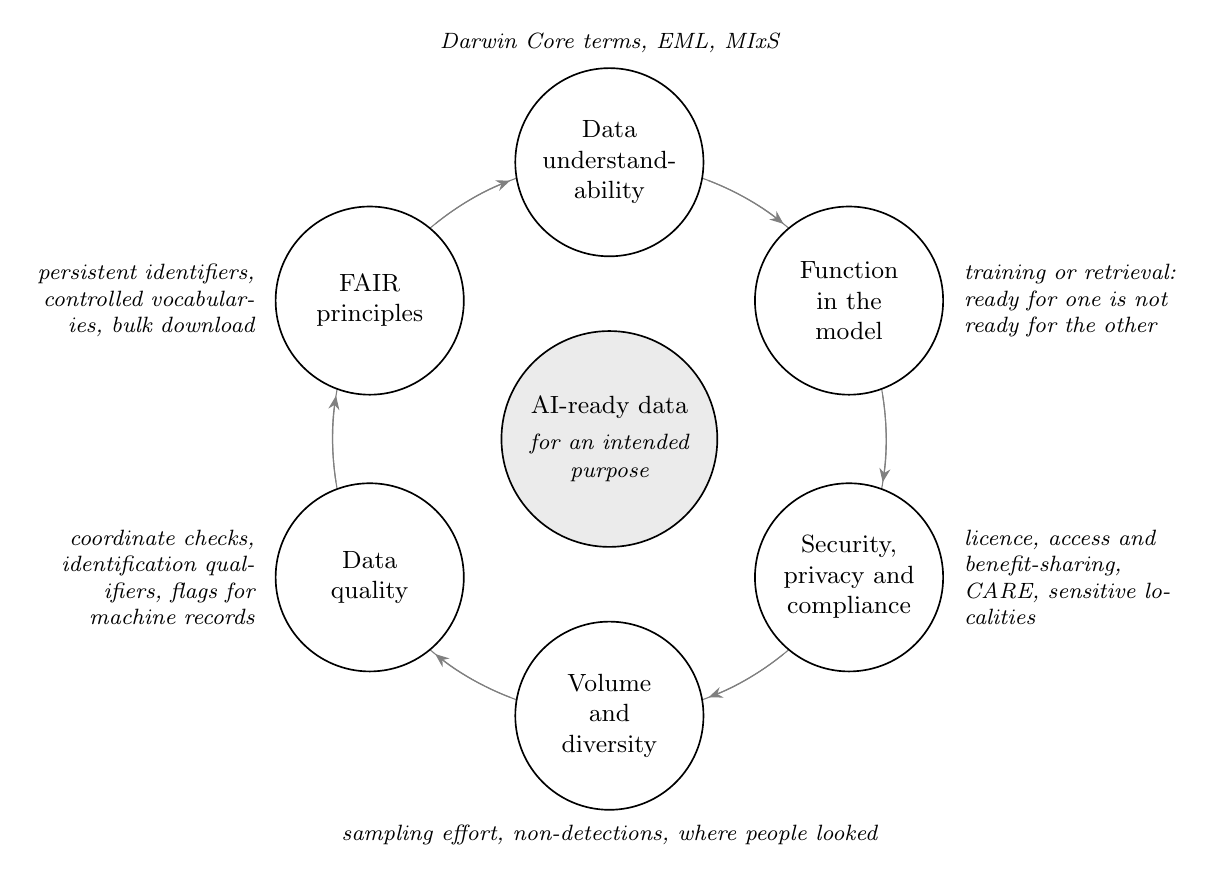
\begin{tikzpicture}[
    dim/.style={draw, circle, minimum size=68pt, inner sep=1pt,
                align=center, fill=white},
    side/.style={note, text width=80pt},
  ]
  \def\R{100pt}
  % the ring: the six depend on one another
  \draw[thin] (0,0) circle[radius=\R];
  \foreach \a in {90,30,-30,-90,-150,150} {
    \draw[thin, ->] ($(0,0)+(\a-21:\R)$)
      arc[start angle=\a-21, end angle=\a-39, radius=\R];
  }
  % centre
  \node[draw, circle, fill=lightgrey, minimum size=78pt, inner sep=1pt,
        align=center] (c) at (0,0)
    {AI-ready data\\[2pt]{\footnotesize\itshape for an intended}\\[-1pt]
     {\footnotesize\itshape purpose}};
  % the six dimensions, clockwise from the top, as in the source
  \node[dim] (u) at (90:\R)   {Data\\understand-\\ability};
  \node[dim] (m) at (30:\R)   {Function\\in the\\model};
  \node[dim] (s) at (-30:\R)  {Security,\\privacy and\\compliance};
  \node[dim] (v) at (-90:\R)  {Volume\\and\\diversity};
  \node[dim] (q) at (-150:\R) {Data\\quality};
  \node[dim] (f) at (150:\R)  {FAIR\\principles};
  % what each means for biodiversity records
  \node[note, above=3pt of u] {Darwin Core terms, EML, MIxS};
  \node[side, right=5pt of m, align=left]
    {training or retrieval: ready for one is not ready for the other};
  \node[side, right=5pt of s, align=left]
    {licence, access and benefit-sharing, CARE, sensitive localities};
  \node[note, below=3pt of v] {sampling effort, non-detections, where people looked};
  \node[side, left=5pt of q, align=right]
    {coordinate checks, identification qualifiers, flags for machine records};
  \node[side, left=5pt of f, align=right]
    {persistent identifiers, controlled vocabularies, bulk download};
\end{tikzpicture}
\end{document}
